\section{Introdução}


\begin{frame}
    \frametitle{Sobre o Artigo}
    \alert{Título:} 3D real-time indoor localization via broadband nonlinear backscatter in
    passive devices with centimeter precision

    \alert{Autores:} Yunfei Ma, Xiaonan Hui Edwin C. Kan, da \alert{Cornell University}

    \alert{Publicado em:} MobiCom '16 Proceedings of the 22nd Annual
    International Conference on Mobile Computing and Networking Pages 216-229

\end{frame}

\begin{frame}
  \frametitle{Contribuições Principais}

    Monitorar a posição de etiquetas RFID no espaço 3D:

    \begin{itemize}
      \item Com \alert{alta precisão} (erro de $3.5$cm)
      \item Em \alert{tempo real}: latência de $0.155$s
      \item Funciona em \alert{ambientes fechados e cheios de objetos}
      \item \alert{Não requer movimento relativo} ou \alert{nós de referência}
    \end{itemize}

    Hardware \& software co-design:

    \begin{itemize}
        \item \alert{Combinação de frequências}
        \item \alert{Modificações no algoritmo HMFCW} (heuristic optimized continuous wave ranging)
        \item Algoritmo de \alert{Localização 3D}
        \item \alert{Tag RFID não-linear}
    \end{itemize}
\end{frame}

\subsection{Aplicações}

\plain{Aplicações}

\begin{frame}
  \frametitle{Interação Humano-Máquina}
  \begin{itemize}
    \item  Controle/monitoração de braços robóticos
  \end{itemize}

  \begin{center}
    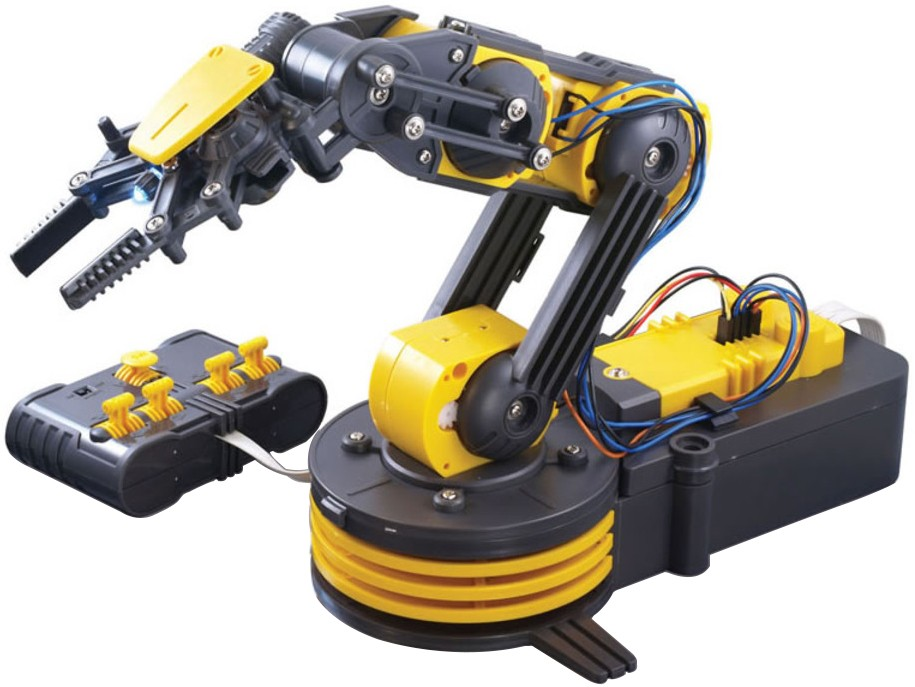
\includegraphics[width=.8\textwidth]{robot-arm}
  \end{center}
\end{frame}

\begin{frame}
  \frametitle{Interação Humano-Máquina}
  \begin{itemize}
    \item  Carros autônomos
  \end{itemize}

  \begin{center}
    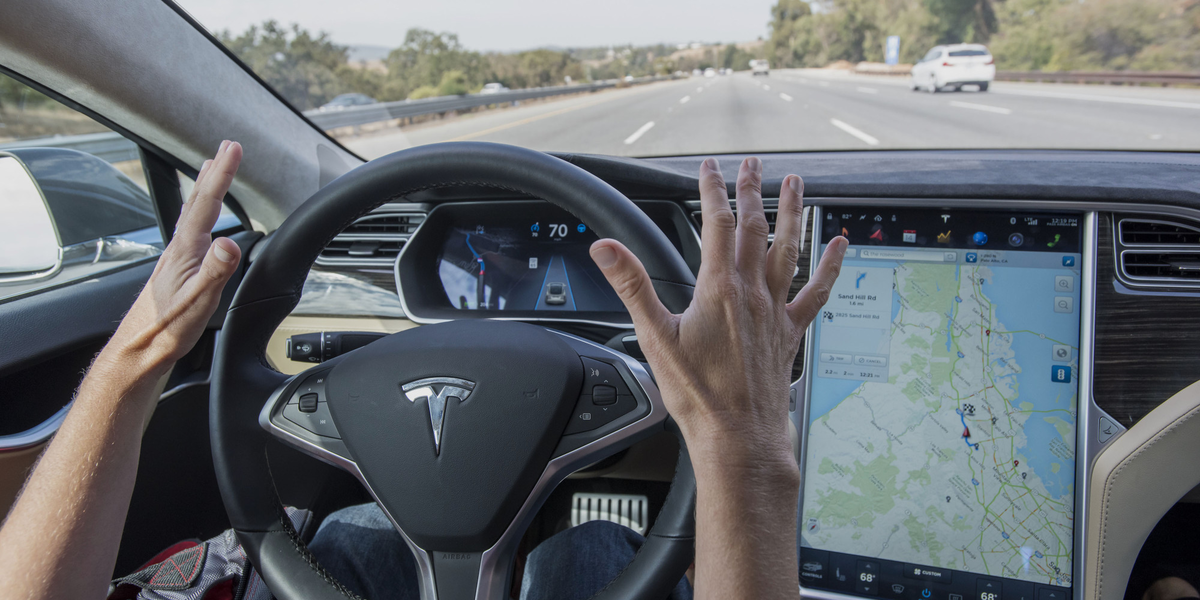
\includegraphics[width=\textwidth]{autopilot}
  \end{center}
\end{frame}

\begin{frame}
    \frametitle{Jogos \& Realidade aumentada}
    \begin{columns}[T,onlytextwidth]
        \column{.5\textwidth}
        \begin{center}
            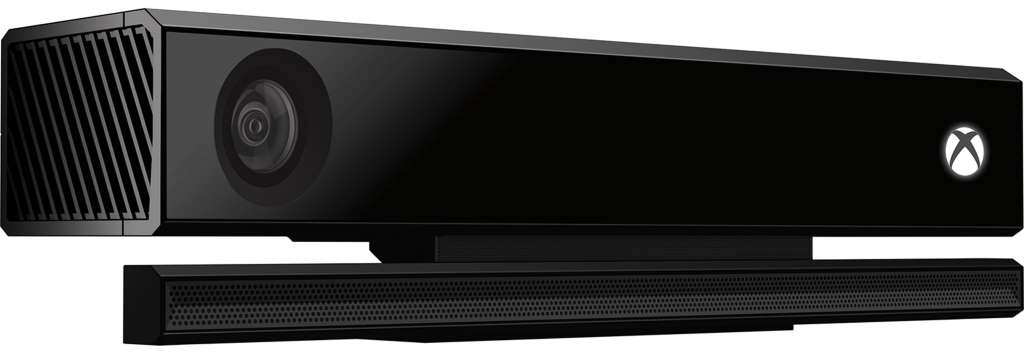
\includegraphics[width=.9\textwidth]{kinect-medium}
        \end{center}

        \column{.5\textwidth}
        \begin{center}
            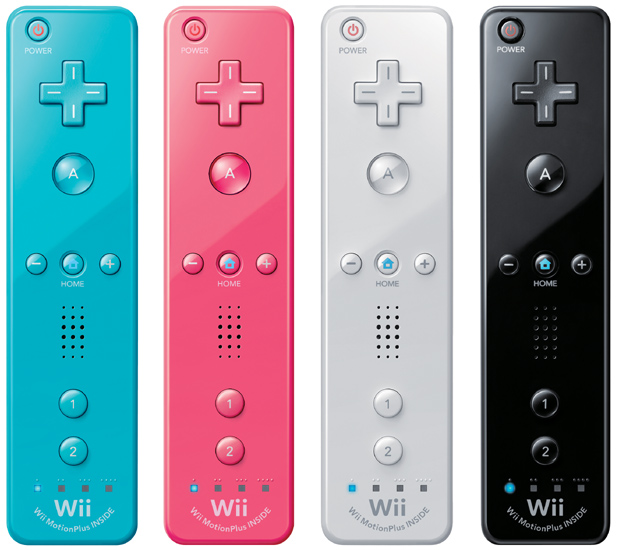
\includegraphics[width=0.5\textwidth]{wii-controller-more}
        \end{center}
    \end{columns}
\end{frame}

\begin{frame}
    \frametitle{Aplicações Comerciais}
        \begin{center}
            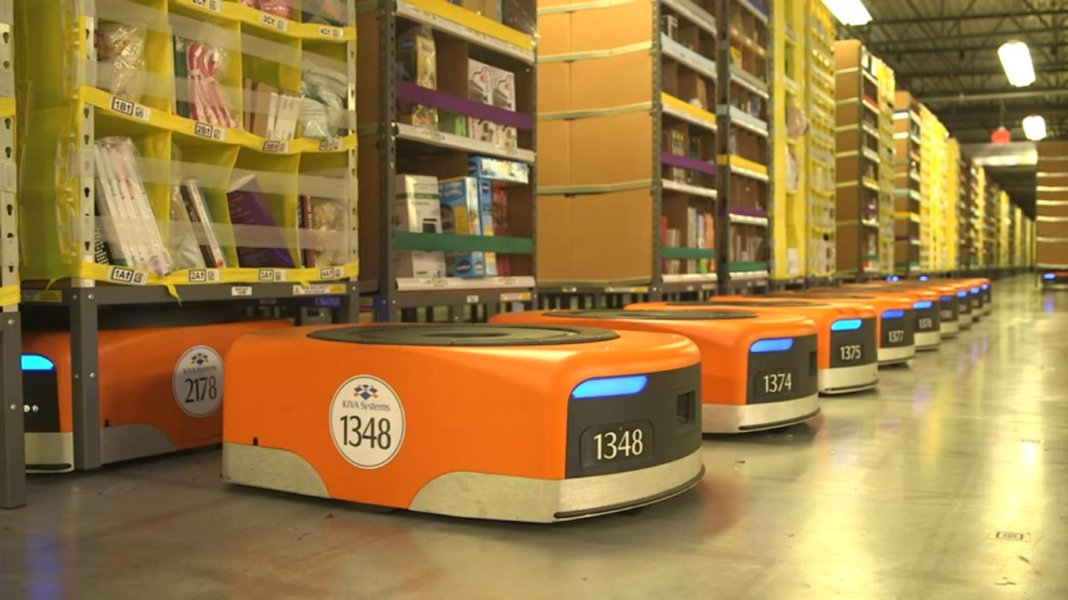
\includegraphics[width=.9\textwidth]{amazon-robots}
        \end{center}
\end{frame}

\begin{frame}
    \frametitle{Aplicações Comerciais}
        \begin{center}
            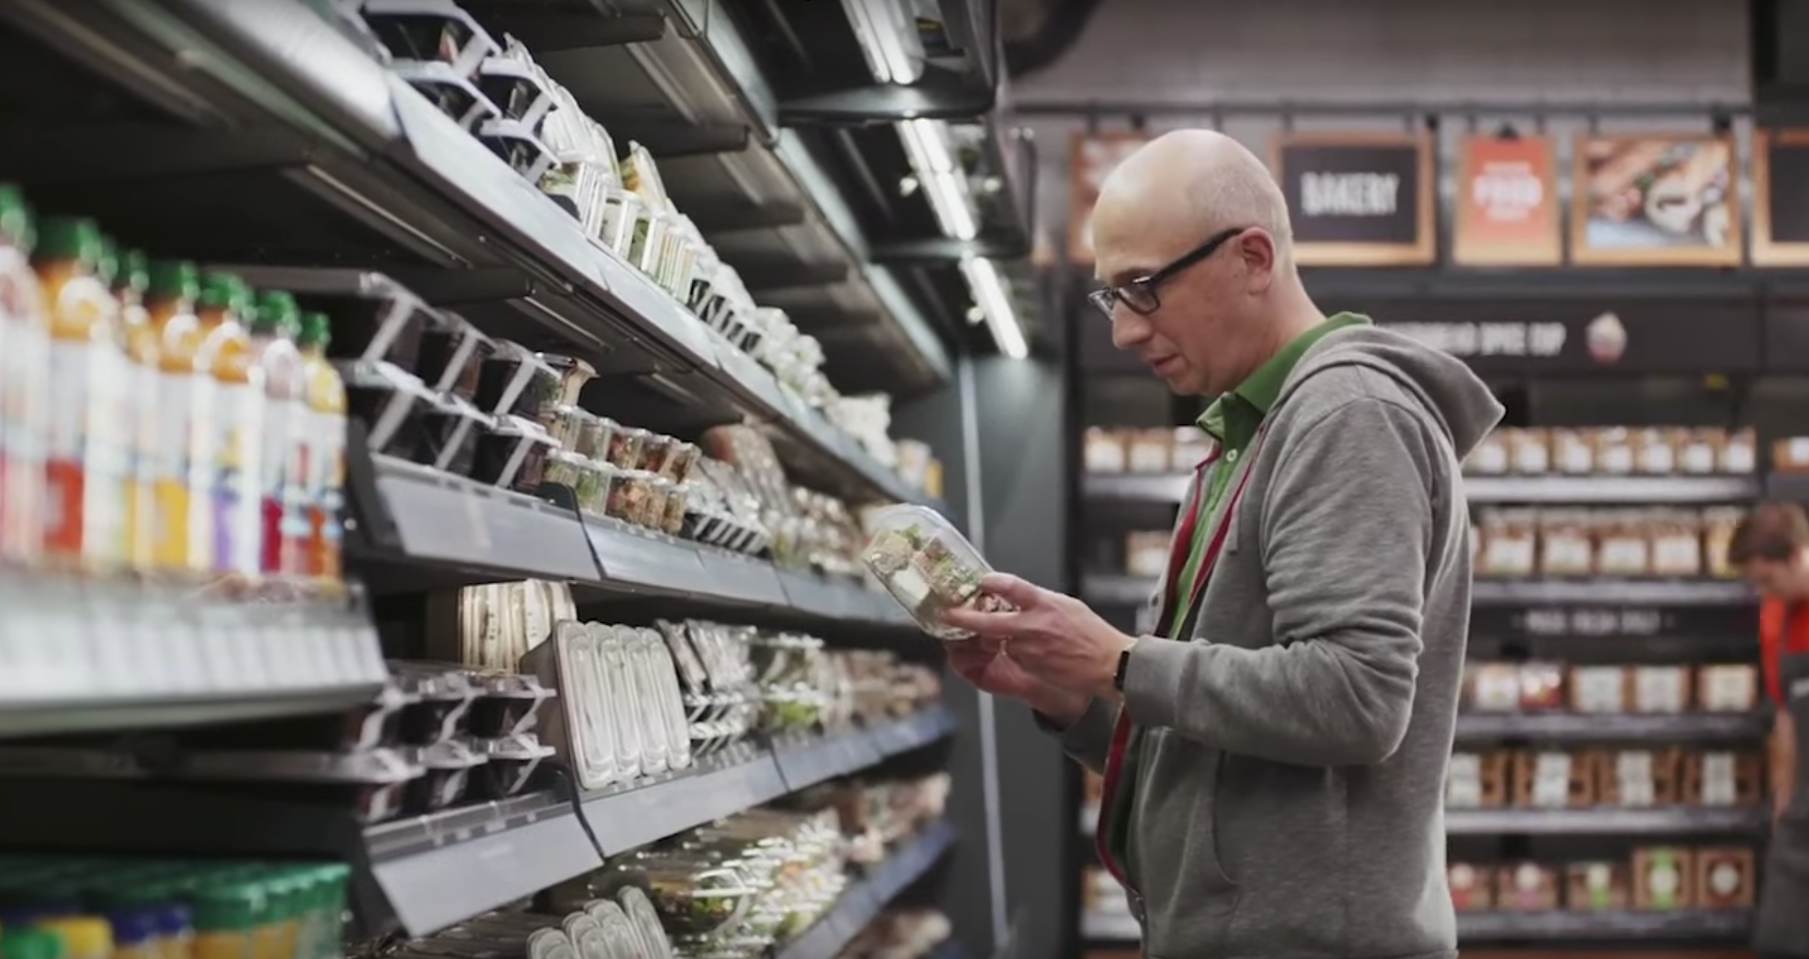
\includegraphics[width=.9\textwidth]{amazon-go-customer}
        \end{center}
\end{frame}

\begin{frame}
  \frametitle{3D-Tracking Hoje}

  Boa parte das técnicas de 3D-Tracking atuais são baseadas em visão
  computacional, com pequenas variações no:

  \begin{itemize}
    \item Aúmero de câmeras utilizadas
    \item Algoritmos de CV utilizados
    \item $\dots$
  \end{itemize}
\end{frame}

\begin{frame}
    \frametitle{Limitações Atuais}

    O problema já não está resolvido?

    \begin{itemize}
    \item  Alta complexidade computacional
    \item  Custo de implementação
    \item  Não funcionam em ambientes com obstáculos
    \end{itemize}

    \begin{center}
        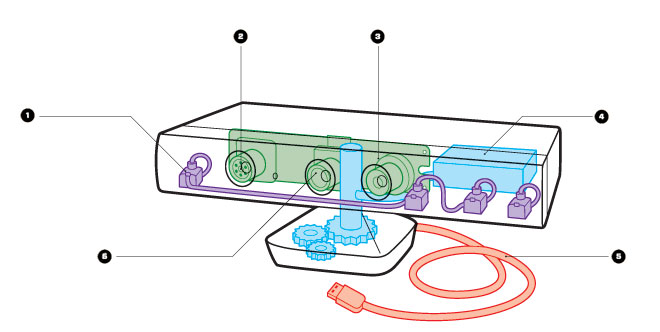
\includegraphics[width=0.8\textwidth]{kinect-diagram}
    \end{center}
\end{frame}


\begin{frame}
    \frametitle{3D-Tracking usando RFIDs}

    Vantagens:
    \begin{itemize}
    \item  \alert{Tags são muito baratas} ($0.1 \sim 0.2$ dólares)!
    \item  Técnica \alert{funciona mesmo com obstáculos}
    \item  \alert{Menor complexidade computacional}!
    \end{itemize}

    Problemas do estado-da-arte que a técnica do artigo supera:
    \begin{itemize}
    \item  Dependência de antenas de referência ou \emph{anchor nodes}
    \item  Dependência de conhecimento prévio da trajetória
    \item  Limitação a 2D-Tracking
    \end{itemize}
\end{frame}
